\documentclass[a4paper,10pt]{article}
\usepackage[utf8]{inputenc}
\usepackage[T1]{fontenc}
\usepackage[margin=0.75in]{geometry}
\usepackage{fancyhdr}
\usepackage{listings}
\usepackage[colorlinks]{hyperref}
\usepackage{amssymb}
\usepackage{graphicx}
\usepackage{listings}
\usepackage{xcolor}
\usepackage{amsmath}
\usepackage{float}
% Alwayws load this last
\usepackage{xcolor}
\usepackage{soul}

\def\chpcolor{blue!60}
\def\chpcolortxt{blue!60}
\def\sectionfont{\sffamily\Large}

\setcounter{secnumdepth}{2}

\makeatletter
%Section:
\def\@sectionstrut{\vrule\@width\z@\@height12.5\p@}
\def\@makesectionhead#1{%
  {\par\vspace{20pt}%
   \parindent 0pt\raggedleft\sectionfont
   \colorbox{\chpcolor}{%
     \parbox[t]{25pt}{\color{white}\@sectionstrut\@depth4.5\p@\hfill
       \ifnum\c@secnumdepth>\z@\thesection\fi}%
   }%
   \begin{minipage}[t]{\dimexpr\textwidth-25pt-2\fboxsep\relax}
   \color{\chpcolortxt}\@sectionstrut\hspace{5pt}#1
   \end{minipage}\par
   \vspace{10pt}%
  }
}
\def\section{\@afterindentfalse\secdef\@section\@ssection}
\def\@section[#1]#2{%
  \ifnum\c@secnumdepth>\m@ne
    \refstepcounter{section}%
    \addcontentsline{toc}{section}{\protect\numberline{\thesection}\textbf{#1}}%
  \else
    \phantomsection
    \addcontentsline{toc}{section}{#1}%
  \fi
  \sectionmark{\textbf{#1}}%
  \if@twocolumn
    \@topnewpage[\@makesectionhead{#2}]%
  \else
    \@makesectionhead{\textbf{#2}}\@afterheading
  \fi
}
\def\@ssection#1{%
  \if@twocolumn
    \@topnewpage[\@makesectionhead{#1}]%
  \else
    \@makesectionhead{#1}\@afterheading
  \fi
}
\makeatother




\makeatletter
\def\@makesubsectionhead#1{%
  {\par\vspace{20pt}%
   \parindent 0pt\raggedleft\sffamily\large
   \ifnum\c@secnumdepth>\z@\color{\chpcolortxt}{\thesubsection}\fi%
   %
   \begin{minipage}[t]{\dimexpr\textwidth-2\fboxsep\relax}
   \vspace{-10pt}\color{black}\hspace{5pt}#1
   \end{minipage}\\[-10pt]
   \noindent\rule{\textwidth}{1pt}\par
   \vspace{10pt}%
  }
}
\def\subsection{\@afterindentfalse\secdef\@subsection\@ssection}
\def\@subsection[#1]#2{%
  \ifnum\c@secnumdepth>\m@ne
    \refstepcounter{subsection}%
    \addcontentsline{toc}{subsection}{\protect\numberline{\thesubsection}\textbf{#1}}%
  \else
    \phantomsection
    \addcontentsline{toc}{subsection}{\textbf{#1}}%
  \fi
  \sectionmark{\textbf{#1}}%
  \if@twocolumn
    \@topnewpage[\@makesubsectionhead{\textbf{#2}}]%
  \else
    \@makesubsectionhead{\textbf{#2}}\@afterheading
  \fi
}
\def\@ssection#1{%
  \if@twocolumn
    \@topnewpage[\@makesubsectionhead{\textbf{#1}}]%
  \else
    \@makesubsectionhead{\textbf{#1}}\@afterheading
  \fi
}
\makeatother



\definecolor{codegreen}{rgb}{0,0.6,0}
\definecolor{codegray}{rgb}{0.5,0.5,0.5}
\definecolor{codepurple}{rgb}{0.58,0,0.82}
\definecolor{backcolour}{rgb}{0.95,0.95,0.92}

%Code listing style named "mystyle"
\lstdefinestyle{mystyle}{
  backgroundcolor=\color{backcolour},   commentstyle=\color{codegreen},
  keywordstyle=\color{magenta},
  numberstyle=\tiny\color{codegray},
  stringstyle=\color{codepurple},
  basicstyle=\ttfamily\footnotesize,
  breakatwhitespace=false,         
  breaklines=true,                 
  captionpos=b,                    
  keepspaces=true,                 
  numbers=left,                    
  numbersep=5pt,                  
  showspaces=false,                
  showstringspaces=false,
  showtabs=true,                  
  tabsize=2
}

%"mystyle" code listing set
\lstset{style=mystyle}


\newcommand{\xhdr}[1]{\vspace{10pt}\noindent{\color{blue!60}\textbf{#1}}}


\newcommand{\task}[1]{\xhdr{ {\large $\mathbf{\blacktriangleright}$} \texttt{TASK #1}}}


\usepackage{tcolorbox}
\newtcolorbox{taskbox}{
    arc=0pt,
    boxrule=1pt,
    colback=gray!10,
    colframe=blue!60,
    width=\textwidth,
    halign=left,
}

\setcounter{section}{-1}




\begin{document}

\sffamily

\begin{center}
\noindent\rule{\textwidth}{1pt}\\[10pt]
{\color{blue!60}{AI539 Natural Language Processing with Deep Learning -- Homework 1}}\\[10pt]
{\LARGE Word Vectors: Distributed Representations of Words}\\[10pt]
{\color{blue!60}{Ameyassh Nagarajan}}\\[10pt]
\noindent\rule{\textwidth}{1pt}
\end{center}

\section{Written Responses}
\vspace{5pt}
\begin{taskbox}
\task{1.1 [2pt]} Implement the \texttt{tokenize} function in \texttt{Vocabulary.py} that processes a string into an array of strings corresponding to tokens. You are free to implement any tokenization schema that eliminates punctuation. If you want to try out lemmitization, the \texttt{nltk} package may be helpful. In your writeup for this question, include a description of what you implemented and include an example input-output pair.
\end{taskbox}
\begin{answerbox}
    \task{1.1 Answer} For the \texttt{tokenize} function I have used the several inbuilt functions in python. To remove the punctuations I have used the following code:
    \newline
    \begin{lstlisting}[language=Python]
        new_text = text.translate(str.maketrans('','',string.punctuation))
    \end{lstlisting}
    
    The tokens are then stored in a list named \texttt{tokens} using the following code:
    \newline
    \begin{lstlisting}[language=Python]
        tokens = new_text.lower().split()
    \end{lstlisting}
\end{answerbox}
\vspace{5pt}

\vspace{5pt}
\begin{taskbox}
\task{1.3 [5pt]} Implement the \texttt{make\_vocab\_charts} function in \texttt{Vocabulary.py} to produce Token Frequency Distribution and Cumulative Fraction Covered charts like those above for your tokenizer and vocabulary cutoff heuristic. We recommend \texttt{matplotlib} for this. Afterwards, running \texttt{build\_freq\_vectors.py} will generate these plots. In your write-up for this question, include these plots and briefly describe the cutoff heuristic you implemented and explain your rational for setting it. 
\end{taskbox}
\begin{answerbox}
    For these figures I have implemented a minimum frequency of 50.\\
    Using a cutoff frequency of 50 allows to ignore words like 'the', 'is', 'and' which might occur frequently. This cuttoff also allows to reduce dimensions which might result in making the model more computationally efficient.
\end{answerbox}
\begin{figure}[h]
    \centering
    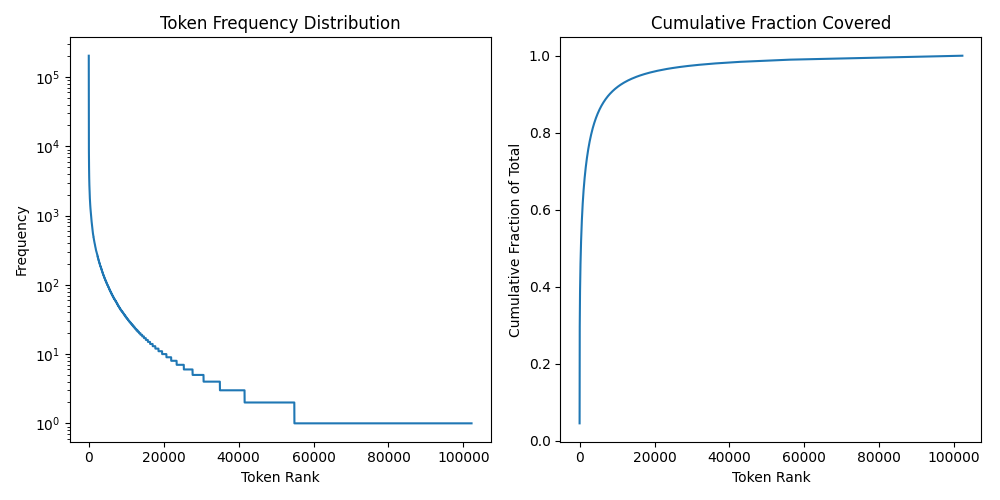
\includegraphics[width=0.5\linewidth]{cumulative_and_freq.png}
    \caption{Cumulative and frequencies}
    \label{fig:enter-label}
\end{figure}
\vspace{5pt}

\vspace{5pt}
\begin{taskbox}
\task{2.1 [5pt]} What are the minimum and maximum values of PMI (Eq.~\ref{eq:pmi})? If two tokens have a positive PMI, what does that imply about their relationship? If they have a PMI of zero? What about if the PMI is negative? Based on your answers, what is an intuition for the use of PPMI?
\end{taskbox}
\begin{answerbox}
    The maximum value of PMI will be positive infinity and the minimum value will be negative infinity. The maximum value is achieved when two words always appear together, and similarly the minimum value is achieved when two words never appear together.\\
    If two token have a positive PMI this indicates that they occur together frequently as opposed to when they have a negative PMI, they do not appear frequently. When two words have a PMI value of $0$ this implies that the two words are independent of each other.\\
    The intiuition for using PPMI is that using words that occur together helps in tasks like semantic analysis in Natural Language Processing.
\end{answerbox}
\vspace{5pt}

\vspace{5pt}
\begin{taskbox}
\task{2.2 [2pt]} Implement the \texttt{compute\_cooccurrence\_matrix} function in \texttt{build\_freq\_vectors.py} which takes a list of article overviews and a vocabulary and produces a co-occurrence matrix $C$. It is up to the student to define what a context is. Note that looping in Python is quite slow such that unoptimized versions of this function can take quite a long time. Feel free to save the result while you are developing to reduce time in future runs (see \texttt{numpy.save/numpy.load}). In your writeup for this task, describe how you defined your context.
\end{taskbox}
\begin{answerbox}
    I have defined the context using a window size of 2. The window size allows the program to refer to two words at the same time. This allows the model to understand what words a single word is being used with frequently.
    The code for my context definition is shown below:
    \begin{lstlisting}[language=Python]
def compute_cooccurrence_matrix(corpus, vocab):
	window_size = 2
	vocab_size = len(vocab.word2idx)
	C = np.zeros((vocab_size, vocab_size), dtype=int)
	word_2_indx = vocab.word2idx

	for s in corpus:
		words= vocab.tokenize(s)
		indx = [word_2_indx.get(word,word_2_indx['UNK']) for word in words]
		for center_indx, center_word in enumerate(indx):
			start = max(0,center_indx - vocab_size)
			end = min(len(indx), center_indx + vocab_size + 1)

			for context in range(start, end, window_size):
				if context != center_indx:
					context_word = indx[context]
					if context_word is not None:
						C[center_word,context_word] += 1

	return C
    \end{lstlisting}
\end{answerbox}
\vspace{5pt}

\vspace{5pt}
\begin{taskbox}
\task{2.4 [10pt]} It has all led up to this! Run \texttt{build\_freq\_vectors.py} and examine the visualized word vectors. You should have semantically meaningful clusters in your plot. Zoom in and identify three such clusters. In your write-up, include an image of each cluster and what category you think it is representing. Also include the plot as a whole.
\end{taskbox}
\begin{answerbox}
    The full plot can be seen in this figure below and three clusters of words can be seen below:
\end{answerbox}
    \begin{figure}[H]
        \centering
        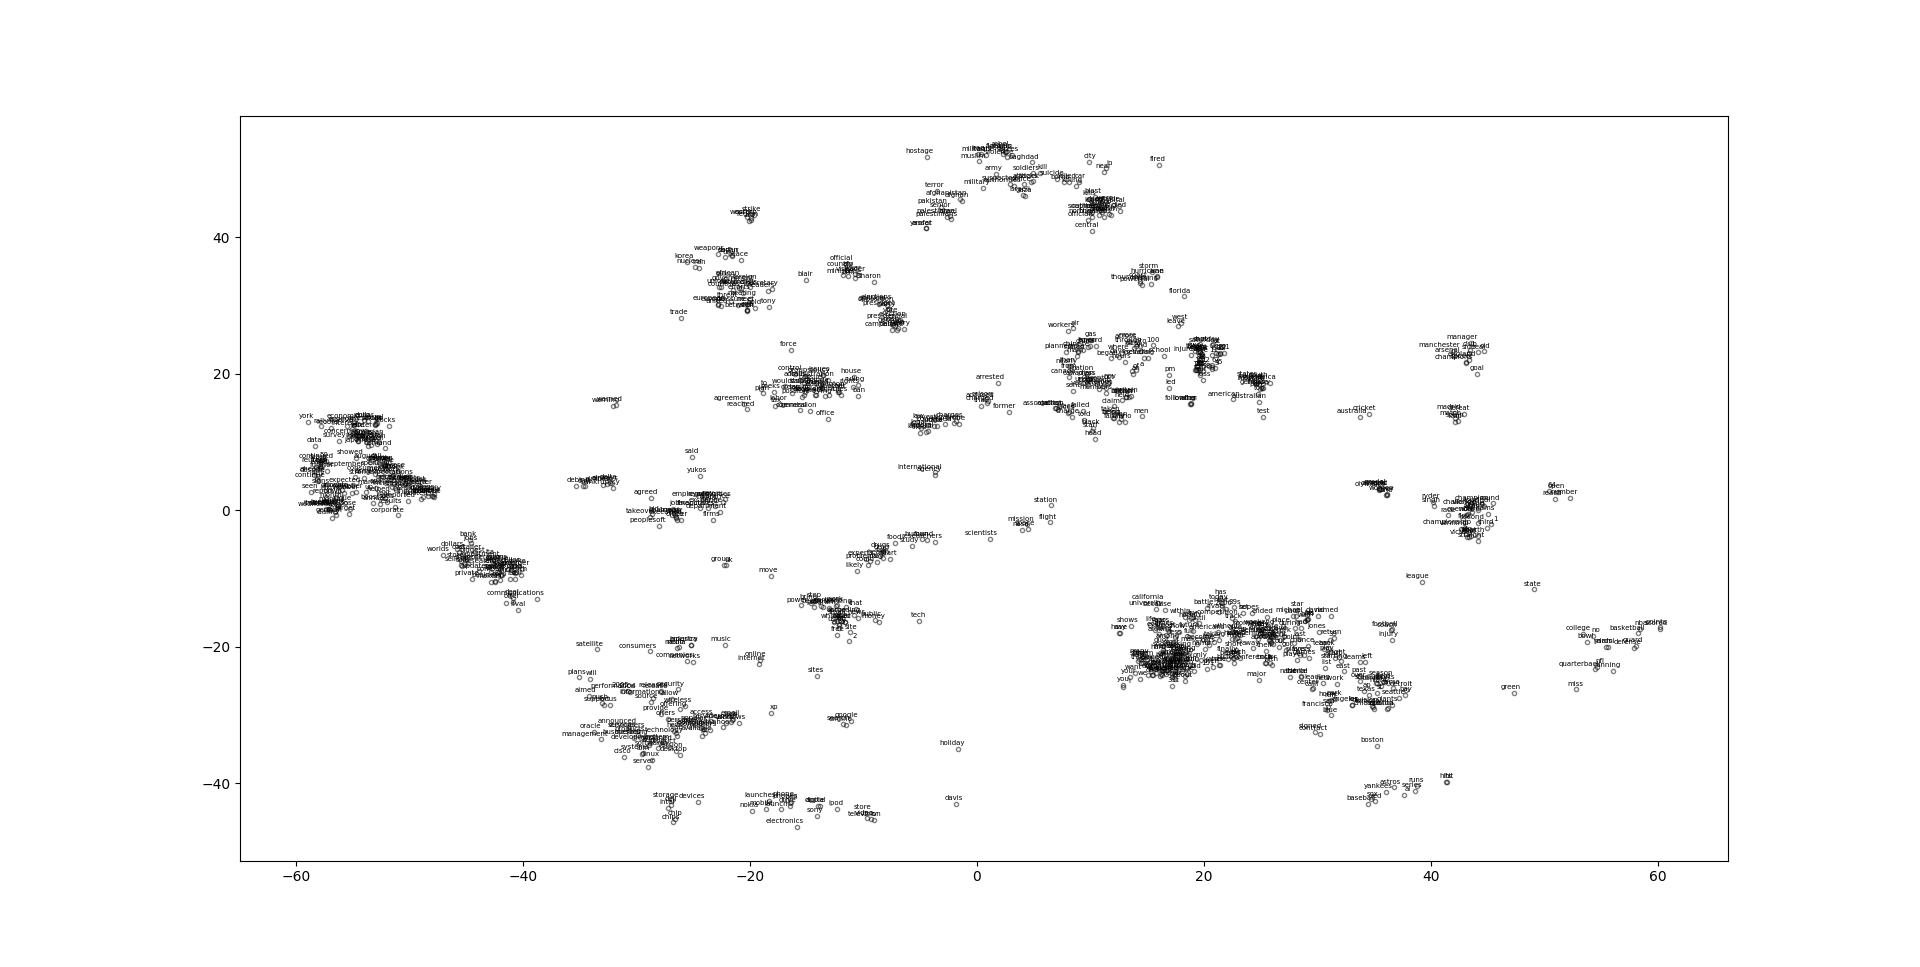
\includegraphics[width=0.5\linewidth]{build_freq.png}
        \caption{Word Vectors}
        \label{fig:enter-label}
    \end{figure}
% \begin{answerbox}
%     Three clusters of words:
% \end{answerbox} 
\begin{figure}[H]
    \centering
    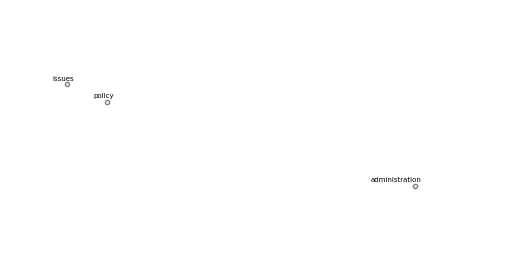
\includegraphics[width=0.5\linewidth]{legislation.png}
    \caption{Cluster representing words related to legislation}
    \label{fig:enter-label}
\end{figure}
\begin{figure}[H]
    \centering
    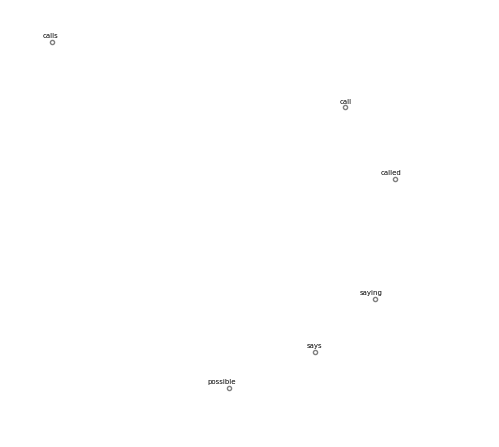
\includegraphics[width=0.5\linewidth]{conversation.png}
    \caption{Words related to a normal conversation}
    \label{fig:enter-label}
\end{figure}
\begin{figure}[H]
    \centering
    
\includegraphics[width=0.5\linewidth]{exec.png}
    \caption{Cluster of words related to executives}
    \label{fig:enter-label}
\end{figure}
\vspace{5pt}

\vspace{5pt}
\begin{taskbox}
\task{3.1 [10pts]} Derive the gradient of the objective $J_B$ in Eq.5 with respect to the model parameters $w_i$, $\tilde{w}_j$, $b_i$, and $\tilde{b}_j$. That is, write the expression for $\nabla_{w_i}J$, $\nabla_{\tilde{w}_j}J$, $\nabla_{b_i}J$, and $\nabla_{\tilde{b}_j}J$. Note that parameters corresponding to words not in $B$ will have zero gradient. 
\end{taskbox} 
\begin{answerbox}
    Given the objective function
\[
J_B = \sum_{(i,j)\in B} f(C_{ij}) \left( \mathbf{w}_i^\top \mathbf{\tilde{w}}_j + b_i + \tilde{b}_j - \log C_{ij} \right)^2,
\]

the gradients with respect to the model parameters are as follows:

\begin{itemize}
    \item Gradient with respect to \( \mathbf{w}_i \):
    \[
    \nabla_{\mathbf{w}_i} J_B = \sum_{j:(i,j)\in B} 2f(C_{ij}) \left( \mathbf{w}_i^\top \mathbf{\tilde{w}}_j + b_i + \tilde{b}_j - \log C_{ij} \right) \mathbf{\tilde{w}}_j
    \]
    
    \item Gradient with respect to \( \mathbf{\tilde{w}}_j \):
    \[
    \nabla_{\mathbf{\tilde{w}}_j} J_B = \sum_{i:(i,j)\in B} 2f(C_{ij}) \left( \mathbf{w}_i^\top \mathbf{\tilde{w}}_j + b_i + \tilde{b}_j - \log C_{ij} \right) \mathbf{w}_i
    \]
    
    \item Gradient with respect to \( b_i \):
    \[
    \nabla_{b_i} J_B = \sum_{j:(i,j)\in B} 2f(C_{ij}) \left( \mathbf{w}_i^\top \mathbf{\tilde{w}}_j + b_i + \tilde{b}_j - \log C_{ij} \right)
    \]
    
    \item Gradient with respect to \( \tilde{b}_j \):
    \[
    \nabla_{\tilde{b}_j} J_B = \sum_{i:(i,j)\in B} 2f(C_{ij}) \left( \mathbf{w}_i^\top \mathbf{\tilde{w}}_j + b_i + \tilde{b}_j - \log C_{ij} \right)
    \]
\end{itemize}

\end{answerbox}
\vspace{5pt}

\vspace{5pt}
\begin{taskbox}
\task{3.3 [5pts]} Run \texttt{build\_glove\_vectors.py} to learn GloVe vectors and visualize them with TSNE! In your write-up, describe how the loss behaved during training (how stably it decreased, what it converged to, etc). Also include the TSNE plot. If everything has been done correctly, you should observe similar clustering behavior as in Task 2.3.
\end{taskbox} 
\begin{answerbox}
    During the training the loss started at about 90\% during the first few epochs and started decreasing as the number of epochs increased. After about 50-60 epochs the loss converged at about 25 to 24\%.
    The TSNE plot can be seen in the figure 6 below:
\end{answerbox}
\begin{figure}[H]
    \centering
    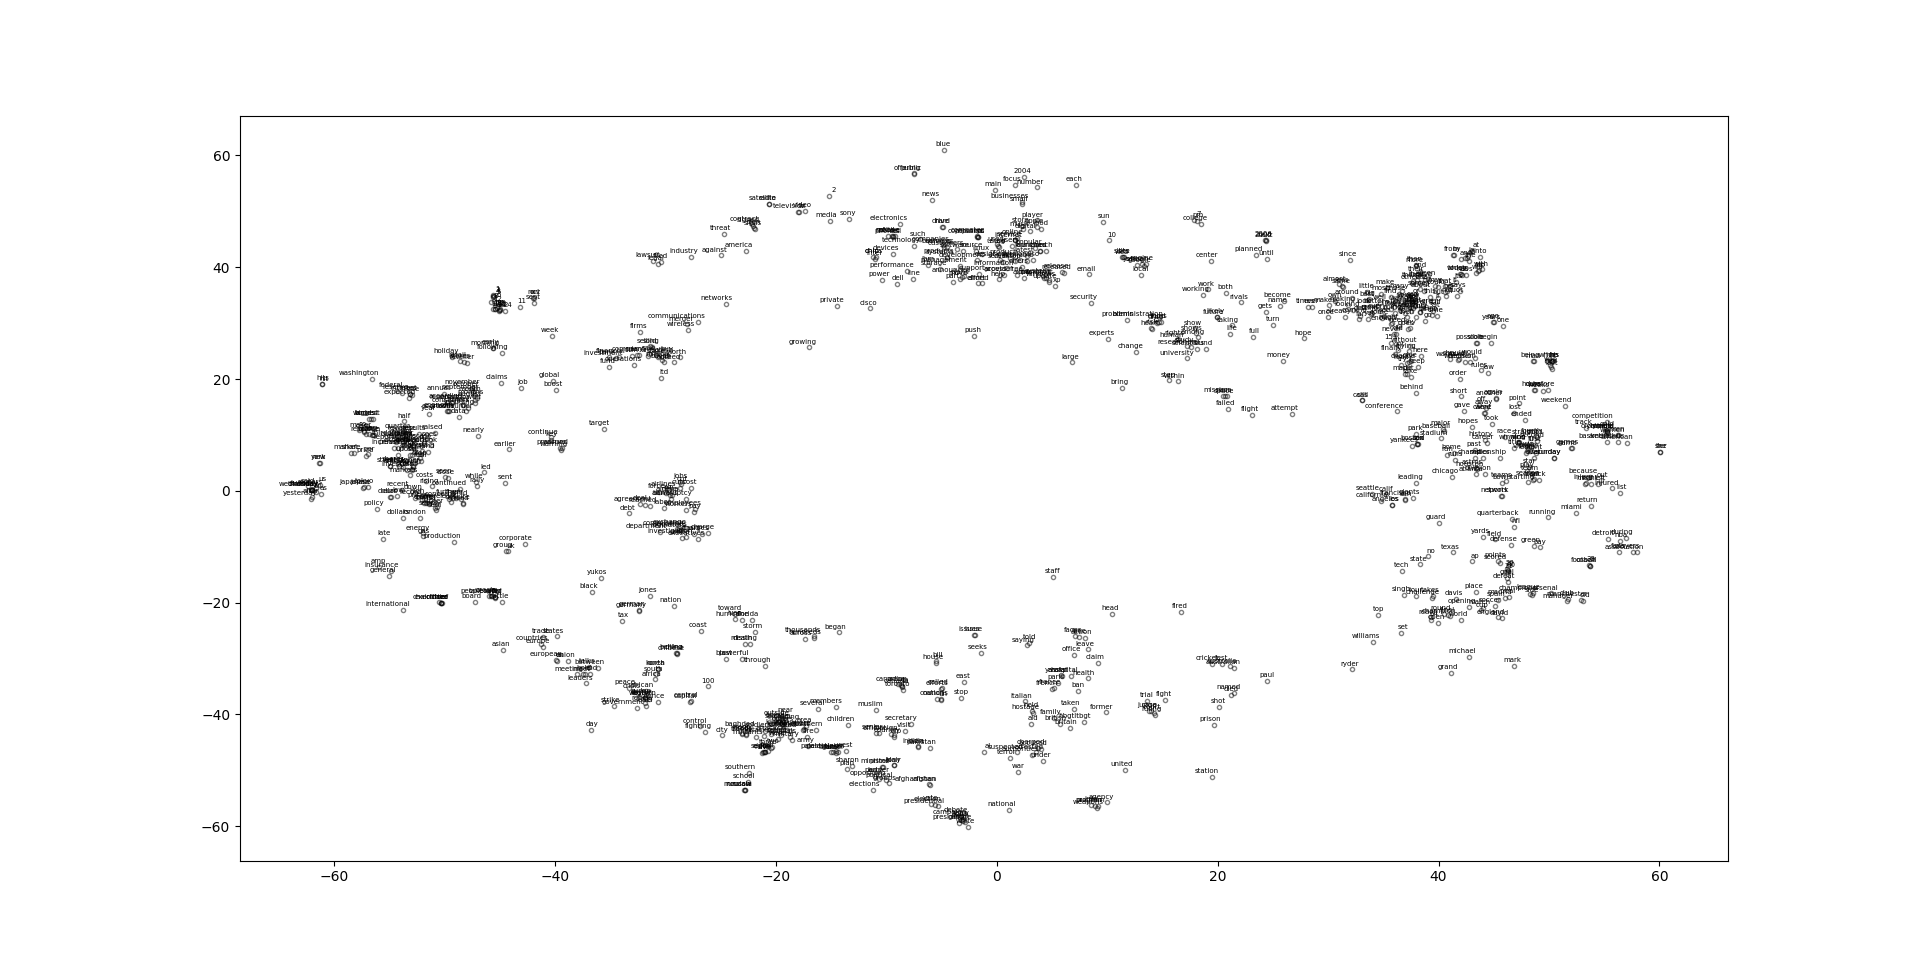
\includegraphics[width=0.5\linewidth]{build_glove_2.png}
    \caption{TSNE Plot}
    \label{fig:enter-label}
\end{figure}
\vspace{5pt}

\vspace{5pt}
\begin{taskbox}
\task{4.1 [3pts]} Use the \texttt{most\_similar} function to find three additional analogies that work. In your response, provide the analogies in the compact \texttt{a:b::c:?} form, the model's list of outputs, and why you consider this output to satisfy the analogy.



\task{4.2 [3pts]} Use the \texttt{most\_similar} function to find three analogies that did not work. In your response to this question, provide the analogies in the compact \texttt{a:b::c:?} form, the model's list of outputs, and why you consider this output to not satisfy the analogy.


\end{taskbox}
\begin{answerbox}
    Some examples where the \texttt{most\_similar} function works are mentioned below
\[
\text{analogy} :  \text{night} : \text{sleep} :: \text{day} : ?
\]
The function \texttt{most\_similar} provides the following potential analogs with their corresponding similarity scores:
\begin{align*}
    \text{naps} & : 0.45, \\
    \text{doze} & : 0.438, \\
    \text{nap} & : 0.434, \\
    \text{restful\_sleep} & : 0.433.
\end{align*}
\[
\text{analogy} :  \text{pen}:\text{book}::\text{tablet}:?
\]
The function \texttt{most\_similar} provides the following potential analogs with their corresponding similarity scores:
\begin{align*}
    \text{ebook} & : 0.524, \\
    \text{e\_reader} & : 0.521, \\
    \text{eBook} & : 0.511.
\end{align*}
\[
\text{analogy} : \text{tiger} :\text{jungle} :: \text{fish}:? 
\]
The function \texttt{most\_similar} provides the following potential analogs with their corresponding similarity scores:
\begin{align*}
    \text{nearshore\_reefs} & 0.499: \\
    \text{mangrove\_swamps} & : 0.496\\
    \text{sandy\_bottoms} & : 0.494
\end{align*}
\end{answerbox}
\begin{answerbox}
Some examples where the function \texttt{most\_similar} does not work:
\[
\text{man} : \text{house} :: \text{monkey} : ?
\]
The function \texttt{most\_similar} provides the following potential analogs with their corresponding similarity scores:
\begin{align*}
    \text{houses} & : 0.458, \\
    \text{monkeys} & : 0.418, \\
    \text{rabbit\_hutch} & : 0.415.
\end{align*}
The function \texttt{most\_similar} provides the following potential analogs with their corresponding similarity scores:
\[
\text{music} : \text{relaxing} ::\text{disturbance} : ?
\]
\begin{align*}
    \text{relaxation} & : 0.485, \\
    \text{Relaxing} & : 0.469, \\
    \text{relax} & : 0.449, \\
    \text{disturbances} & : 0.44.
\end{align*}
\[
\text{apple} : \text{healthy} :: \text{ice\_cream} : ?
\]
The function \texttt{most\_similar} provides the following potential analogs with their corresponding similarity scores:
\begin{align*}
    \text{healthier} & : 0.491, \\
    \text{heathy} & : 0.483, \\
    \text{eating\_nutritious\_foods} & : 0.451.
\end{align*}
\end{answerbox}
\vspace{5pt}

\vspace{5pt}
\begin{taskbox}
\task{4.3 [2pts]} Use the \texttt{most\_similar} function to find two additional cases of bias based on gender, politics, religion, ethnicity, or nationality. In your response, provide the analogies in the compact \texttt{a:b::c:?} form, the model's list of outputs for both \texttt{a:b::c:?} and \texttt{c:b::a:?}, and why you consider this output to be biased based on the model's two responses.


\task{4.4 [2pts]} Why might these biases exist in \texttt{word2vec} and what are some potential consequences that might result if \texttt{word2vec} were used in a live system?
\end{taskbox}
\vspace{5pt}
\begin{answerbox}
    Examples where the function \texttt{most\_similar} shows bias can be seen here\\
    \end{answerbox}
    \begin{answerbox}
        
    Consider the analogy:
\[
\text{man} : \text{earns} :: \text{woman} : ?
\]
\begin{align*}
    \text{receives} & : 0.633, \\
    \text{garners} & : 0.597, \\
    \text{earn} & : 0.566.
\end{align*}
These results may include bias related to gender roles that are present in the model's training corpus.\\
\end{answerbox}
\begin{answerbox}
Consider the analogy:
\[
\text{man} : \text{handsome} :: \text{woman} : ?
\]
\begin{align*}
    \text{shapely} & : 0.556, \\
    \text{comely} & : 0.534, \\
    \text{bosomy} & : 0.524, \\
    \text{curvacious} & : 0.518.
\end{align*}
These results highlights bias in describing the physical features of a man and a woman.
\end{answerbox}

\begin{answerbox}
    Consider the analogy:
\[
\text{dress} : \text{good} :: \text{burkha} : ?
\]
\begin{align*}
    \text{bad} & : 0.499, \\
    \text{decent} & : 0.494, \\
    \text{excellent} & : 0.484.
\end{align*}
These results reflect how there is a bias based on religion.
\end{answerbox}
\begin{answerbox}
    One of the reasons why these biases might exist in word2vec is mainly because of the kind of data it trains on and the associations made in the data for particular words. As word2vec uses context to learn word association, the way in which these words are used plays a role in the bias that is inherited by the model.
    \\
    Potential issues that might arise as a result of this bias is the reinforcement of stereotypes, biases can reinforce stereotypes which might result in limited visibility to underrepresented individuals. Bias might also lead to flaws in decision making as bias might influence a live systems decision making which might lead to potential unfair treatement.
\end{answerbox}
\begin{comment}
\pagebreak


\begin{center}
\noindent\rule{\textwidth}{1pt}\\[10pt]
{\color{blue!60}{AI539 Natural Language Processing with Deep Learning -- Homework 1}}\\[10pt]
{\LARGE Word Vectors: Distributed Representations of Words}\\[10pt]
\noindent\rule{\textwidth}{1pt}
\end{center}

\noindent\textbf{Overview and Objectives.} This assignment will cover the basics of processing text (simple tokenization and vocabulary building) and distributional representations of words. We will learn our own word vectors from a training corpus and examine what relationships have been learned in our small-scale problem. Finally, we will take a look at \texttt{word2vec} \cite{mikolov2013efficient} word vectors learned on large-scale data and identify some implicit biases captured in training.\\

\noindent\textbf{How to Do This Assignment.} The assignment walks you through completing the provided skeleton code and analyzing some of the results. Anything requiring you to do something is marked as a "Task" and has associated points listed with it. You are expected to turn in both your code and a write-up answering any task that requested written responses. Submit a zip file containing your completed skeleton code and a PDF of your write-up to Canvas. 

To ensure you have the right packages, run \texttt{pip install -r requirements.txt} in the skeleton code folder.\\

\noindent\textbf{Advice.} Start early. Students will need to become familiar with \texttt{numpy} and \texttt{matplotlib} for this and future assignments. 

\section{Getting Used to Handling Language Data [10pt]}
%\subsection{AG News Dataset}
We will be using the AG News Benchmark \cite{Zhang2015CharacterlevelCN} dataset as our data source for this homework. \href{http://groups.di.unipi.it/~gulli/AG_corpus_of_news_articles.html}{AG News} is a collection of over a million news articles scraped from over 2000 news sources. The AG News Benchmark \cite{Zhang2015CharacterlevelCN} is a 120,000 article subset of these covering four topics ( World / Sports / Business / Technology ) and is used as a benchmark for text classification. The benchmark retains only the article titles and overviews. 
%
The skeleton code file \texttt{build\_freq\_vectors.py} already loads this dataset based on the HuggingFace dataset package API (\texttt{pip install datasets}). It will download the dataset the first time it is run.
%
\begin{center}
\begin{minipage}{0.8\textwidth}
\begin{lstlisting}[language=Python, caption=Code to load the AG News Dataset]
from datasets import load_dataset
...
dataset = load_dataset("ag_news")
\end{lstlisting}
\end{minipage}
\end{center}
%
The \texttt{dataset} structure returned looks like this
%
\begin{center}
\begin{minipage}{0.8\textwidth}
\begin{lstlisting}[language=Python, caption=AG News Dataset structure]
DatasetDict({
    train: Dataset({
        features: ['text', 'label'],
        num_rows: 120000
    })
    test: Dataset({
        features: ['text', 'label'],
        num_rows: 7600
    })
}
\end{lstlisting}
\end{minipage}
\end{center}
%
and contains article \texttt{text} and \texttt{label} for 120,000 training instances and 7600 test instances.


\subsection{Building a Token Vocabulary}


\xhdr{Tokenization.} It is often easier to consider text as a sequence of discrete tokens. The process of converting a string to such a sequence is known as tokenization. Given a sentence like ``The quick, brown fox jumped over the lazy dog'', one possible tokenization is to ignore punctuation and capitalization then break on white-space as below.
%
\begin{center}
\begin{minipage}{0.95\textwidth}
\begin{lstlisting}[language=Python]
> vocab.tokenize("The quick, brown fox jumped over the lazy dog.")
["the", "quick", "brown", "fox", "jumped", "over", "the", "lazy","dog"]
\end{lstlisting}
\end{minipage}
\end{center}
%
Basing a system on these tokens is fine, but it is a design decision. For instance -- conjugations such as \texttt{jumped}, \texttt{jump}, and \texttt{jumps} would all be different tokens despite having common root meanings, as would any misspellings (\texttt{jupmed}). Alternative tokenizations include sub-word tokenization (\texttt{jumped} $\rightarrow$ \texttt{[jump}, \texttt{ed]}) or pre-processing with \emph{lemmitization} to reduce words to their roots (\texttt{jumped} $\rightarrow$ \texttt{[jump]}, \texttt{are} $\rightarrow$ \texttt{[be]}). Lemmitization has its own drawbacks -- possibly merging different word-senses, potentially resulting in poor specificity (i.e.~can't tell \texttt{jump} from \texttt{jumping}).

\vspace{5pt}
\begin{taskbox}
\task{1.1 [2pt]} Implement the \texttt{tokenize} function in \texttt{Vocabulary.py} that processes a string into an array of strings corresponding to tokens. You are free to implement any tokenization schema that eliminates punctuation. If you want to try out lemmitization, the \texttt{nltk} package may be helpful. In your writeup for this question, include a description of what you implemented and include an example input-output pair.
\end{taskbox}
\vspace{5pt}

\xhdr{Vocabulary.} Estimates suggest there are millions of words in active use in English; however, we are unlikely to encounter the vast, vast majority of them in our limited dataset. For efficiency, it is common practice to consider only frequent tokens in the training corpus -- common heuristics include taking the most frequent $k$ tokens, taking only tokens that occur at least $n$ times, or taking as many words as necessary to cover X\% of the total token occurrences. 
%
%
\begin{center}
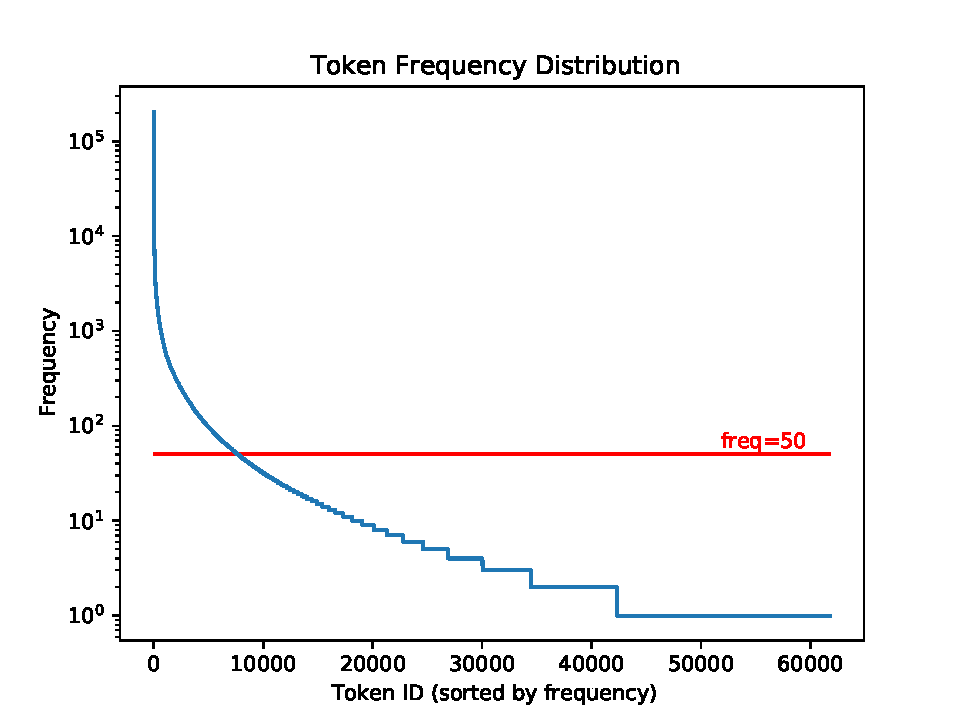
\includegraphics[width=0.495\textwidth]{figures/freq.pdf}\hfill
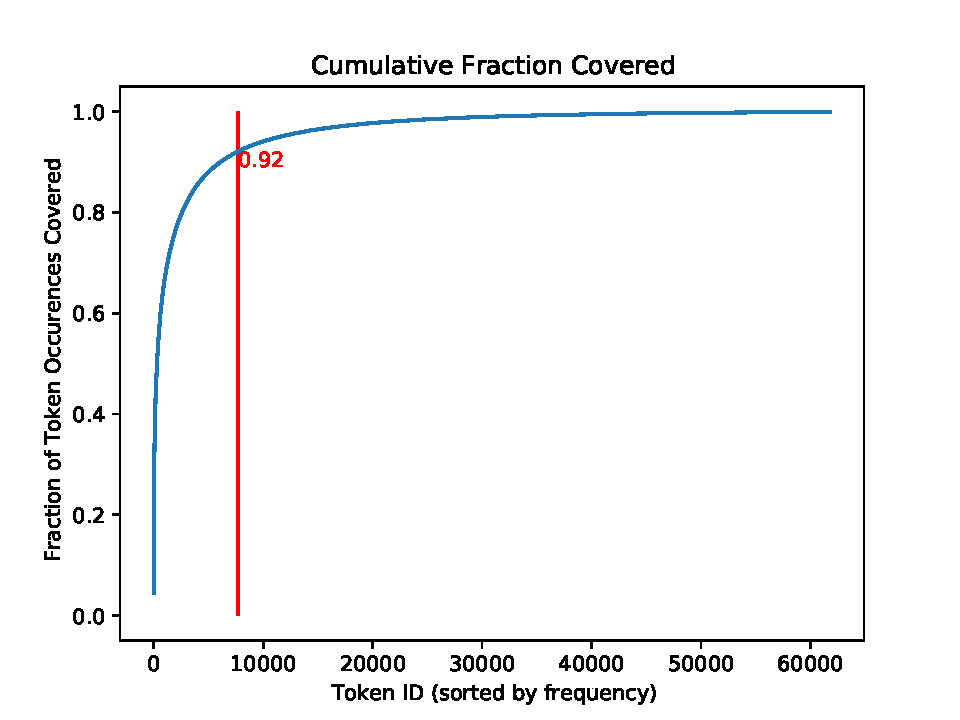
\includegraphics[width=0.495\textwidth]{figures/cover.pdf}
\end{center}
%
%
The above plots show the effect of cutting off our vocabulary by selecting only tokens with greater than 50 occurrences. The frequency distribution plot (left) has a log-scale for the y-axis and demonstrates the \emph{long-tail} property of language. A few tokens are used very frequently but very many tokens are used rarely. The right plot shows the cumulative fraction of word occurrences covered. That is to say,  if the vocabulary is cut off at the $i$th word on the x-axis, the curve shows what fraction of the total number of tokens appearing in the training set (including all instances) would have a corresponding word in the vocabulary. The line marked in red corresponds to a \texttt{freq=50} cutoff and captures 92\% of the tokens in the dataset. As is common practice, we consider the other 8\% of tokens (and any new ones we see at test time) to correspond to a special \texttt{UNK} token in our vocabulary. 

Finally, it is often easier to deal with sequences of tokens as indexes into our vocabulary rather than as raw text (We'll see this in the next section and in later homeworks). That is, if we have the following vocabulary:
%
\begin{center}
\begin{minipage}{0.95\textwidth}
\begin{lstlisting}[language=Python]
["the", "brown", "fox", 'dish", "spoon", "over", "jumped", "lazy","dog", "UNK"]
\end{lstlisting}
\end{minipage}
\end{center}
%
Then the index-represented tokenization of "The quick, brown fox jumped over the lazy dog" would be:
%
\begin{center}
\begin{minipage}{0.95\textwidth}
\begin{lstlisting}[language=Python]
> vocab.textToIdx(vocab.tokenize("The quick brown fox jumped over the lazy dog."))
[0, 9, 1, 2, 6, 5, 0, 7, 8]

> vocab.idxToText([0, 9, 1, 2, 6, 5, 0, 7, 8])
["The", "UNK", "brown", "fox", "jumped", "over", "the", "lazy", "dog"]
\end{lstlisting}
\end{minipage}
\end{center}
%
Notice that the vocabulary did not include the word \texttt{quick} and so this token was mapped to \texttt{UNK}. To make these operations simple, most implementations build two indexes -- \texttt{word2idx} and \texttt{idx2word} -- which map between the two representations via a simple lookup.


\vspace{5pt}
\begin{taskbox}
\task{1.2 [3pt]} Implement the \texttt{build\_vocab} function in \texttt{Vocabulary.py} which constructs a finite vocabulary from a string containing all the text from the training corpus. This includes implementing some heuristic for thresholding the number of words and building the \texttt{word2indx} and \texttt{idx2word} indexes.


\task{1.3 [5pt]} Implement the \texttt{make\_vocab\_charts} function in \texttt{Vocabulary.py} to produce Token Frequency Distribution and Cumulative Fraction Covered charts like those above for your tokenizer and vocabulary cutoff heuristic. We recommend \texttt{matplotlib} for this. Afterwards, running \texttt{build\_freq\_vectors.py} will generate these plots. In your write-up for this question, include these plots and briefly describe the cutoff heuristic you implemented and explain your rational for setting it. 
\end{taskbox}
\vspace{5pt}

\section{Frequency-Based Word Vectors -- PPMI [20pts]}

As we discussed in class, the distributional hypothesis suggests a word's meaning can be derived from how it is used with other words in natural language. In order to follow this philosophy, we must first define some notion of the relationship between words in text. One option is to use raw co-occurrence statistics, but as we noted in class this results in large, sparse vectors and frequent words can dominate similarity calculations. 

\subsection{Pointwise Mutual Information (PMI) Matrix}
First used in NLP in 1990 \cite{church1990word}, pointwise mutual information (PMI) has been widely applied in word similarity tasks. Let $p(w_i, w_j)$ be the probability of tokens $w_i$ and $w_j$ co-occurring in any context and let $p(w_i)$ be the probability of observing token $w_i$ in any context. We can then define the pointwise mutual information between tokens $w_i$ and $w_j$ as:

\begin{equation}
    \mbox{PMI}(w_i,w_j) = \log \frac{p(w_i, w_j)}{p(w_i)p(w_j)}
    \label{eq:pmi}
\end{equation}

\noindent Commonly, practitioners will clip PMI values less than zero. The resulting function is referred to as Positive Pointwise Mutual Information (PPMI) and can be written as $\mbox{PPMI}(w_i, w_j) = \max(0, \mbox{PMI}(w_i, w_j)$.

\vspace{5pt}
\begin{taskbox}
\task{2.1 [5pt]} What are the minimum and maximum values of PMI (Eq.~\ref{eq:pmi})? If two tokens have a positive PMI, what does that imply about their relationship? If they have a PMI of zero? What about if the PMI is negative? Based on your answers, what is an intuition for the use of PPMI?
\end{taskbox}
\vspace{5pt}


\xhdr{Estimating PPMI.} Computing an estimate for PPMI from a dataset is straight-forward given co-occurrence statistics. Consider a dataset of $N$ text contexts. A context could be a whole document, paragraph, sentence, or even small windows in text (e.g.~"The dog jumped over the moon." $\rightarrow$ "The dog jumped", "dog jumped over", "jumped over the", "over the moon"). The scale of these contexts determine our notion of relatedness. Often word vector learning algorithms will use a small window of text.


Let $C$ be a matrix of co-occurence counts such that the $ij$th element of C  denoted $C_{ij}$ is the number of times both $w_i$ and $w_j$ occur in a context. Note that the diagonals  of this matrix ($C_{ii}$) count the number of contexts in which each token occurs. We can then compute
%
\begin{equation}
    \mbox{PPMI}(w_i,w_j) = \max\left(0,~~\log\frac{C_{ij}N}{C_{ii}C_{jj}}\right)
\end{equation}
%
We can store these PPMI values in a matrix $P$ such that $P_{ij} = \mbox{PMI}(w_i, w_j)$. 

\vspace{5pt}
\begin{taskbox}
\task{2.2 [2pt]} Implement the \texttt{compute\_cooccurrence\_matrix} function in \texttt{build\_freq\_vectors.py} which takes a list of article overviews and a vocabulary and produces a co-occurrence matrix $C$. It is up to the student to define what a context is. Note that looping in Python is quite slow such that unoptimized versions of this function can take quite a long time. Feel free to save the result while you are developing to reduce time in future runs (see \texttt{numpy.save/numpy.load}). In your writeup for this task, describe how you defined your context.

\task{2.3 [3pt]} Implement the \texttt{compute\_ppmi\_matrix} function in \texttt{build\_freq\_vectors.py} which calls \texttt{compute\_cooccurrence\_matrix} and then computes a PPMI matrix given a list of article overviews and a vocabulary.  \emph{Hint: Add a small constant to $C$ to avoid problems with $\log(0)$.}
\end{taskbox}
\vspace{5pt}


\xhdr{Our First Word Vector.} A single row $P_{i:}$ of this PPMI matrix corresponds to a vector of PPMI values between token $w_i$ and all other tokens. This is our first distributed word vector; however, it is quite large and mostly sparse such that distances between words vectors in this high of a dimension are unlikely to be very meaningful. 


\subsection{Dimensionality Reduction and Visualization}

\xhdr{Dimensionality Reduction with Truncated SVD.} To reduce the dimensionality of our word vectors, we apply Truncated Singular Value Decomposition. Truncated SVD of a matrix $A$ finds a $k$-rank matrix $D$ such that $||D-A||_F$ is minimized. Specifically, $D$ has the form $D=U\Sigma V^T$ where $\Sigma$ is a diagonal matrix of the $k$ largest singular values. Following \cite{levy2014neural}, we take our final word vectors as $[U\Sigma^{1/2}, V\Sigma^{1/2}]$ where $[\cdot, \cdot]$ denotes concatenation. This is already implemented in the \texttt{dim\_reduce} function in \texttt{build\_freq\_vectors.py}.

\xhdr{Visualizing Word Vectors.} To visualize our word vectors in 2D, the code applies T-SNE \cite{maaten2008visualizing}. T-SNE is a non-linear dimensionality reduction method commonly used to display word vectors and other high-dimensional data. The \texttt{plot\_word\_vectors\_tsne} function in \texttt{build\_freq\_vectors.py} is already set up to produce this visualization. An example visualization from our run is below.
%
\begin{center}
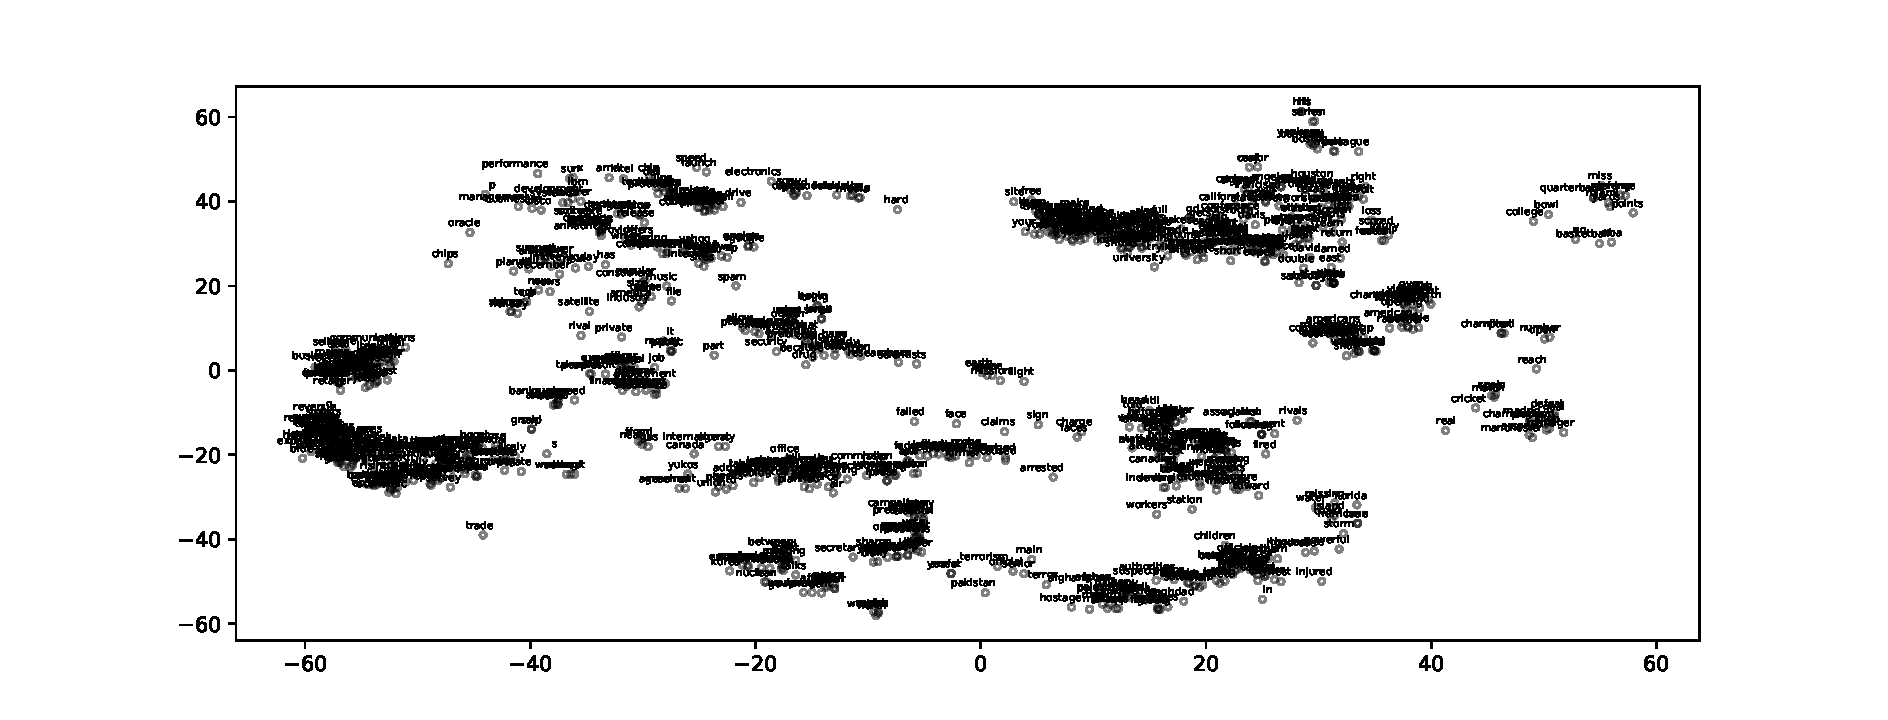
\includegraphics[width=\textwidth]{figures/wordvectors.pdf}
\end{center}
%
It is pretty messy at this resolution but zooming in on the clusters shows the semantics we've learned. For instance, the small middle-right cluster corresponds to soccer and includes words like \emph{''arsenal, manchester, madrid, soccer, england, side, club, manager, goal, defeat, spain, cup, match, ...``}. If you make different choices about tokenization, vocabulary, or the scale of your contexts than we did -- your generated plot will be different.

\vspace{5pt}
\begin{taskbox}
\task{2.4 [10pt]} It has all led up to this! Run \texttt{build\_freq\_vectors.py} and examine the visualized word vectors. You should have semantically meaningful clusters in your plot. Zoom in and identify three such clusters. In your write-up, include an image of each cluster and what category you think it is representing. Also include the plot as a whole.
\end{taskbox}
\vspace{5pt}

\newpage
\section{Learning-Based Word Vectors -- GloVe [25pts]}
As discussed in lecture, an alternative approach is to assume word co-occurrence can be modelled purely as an interaction between word vectors. This approach is taken by popular algorithms like \texttt{word2vec}\cite{mikolov2013efficient} and GloVe \cite{pennington2014glove}. In this section, we'll implement the GloVe algorithm in our setting.

The GloVe algorithm poses the problem as a weighted log bilinear regression problem wherein interactions between word vectors should be predictive of the log of their co-occurrence frequency. As before, let $C$ be a matrix of co-occurrence counts. The GloVe objective can be written as a sum of weighted squared error terms for each word-pair in a vocabulary,
%
\begin{equation}
    J = \overbrace{\sum_{i,j  \in V}}^{\mbox{\shortstack{sum over\\ word pairs}}} \underbrace{f(C_{ij})}_{\mbox{weight}} ~~~( \overbrace{w_i^T\tilde{w}_j + b_i + \tilde{b}_j - \log C_{ij}}^{\mbox{error term}})^2
    \label{eq:glove}
\end{equation}
%
where each word $i$ is associated with word vector $w_i$, context vector $\tilde{w}_i$, and word/context biases $b_i$ and $\tilde{b}_i$.  Unlike word2vec which we studied in class, this objective does not sum over a corpus, but rather over pairs of words in the vocabulary. The $f(C_{ij})$ term is a weighting to avoid frequent co-occurrences from dominating the objective and is defined as
\begin{equation}
    f(X_{ij}) = min(1, C_{ij}/100)^{0.75}
\end{equation}
%
To minimize this objective, \texttt{build\_glove\_vectors.py} implements a simple stochastic gradient descent with momentum optimization algorithm; however, it is missing the expressions for the gradients.
Given a batch of word-pairs $B = \{ (i_m,j_m)\}_{m=1}^M$, we can write the per-batch objective as:

\begin{equation}
    J_B = \sum_{ (i_m,j_m)  \in B} f(C_{i_m j_m})( w_{i_m}^T\tilde{w}_{j_m} + b_{i_m} + \tilde{b}_{j_m} - \log C_{i_m j_m})^2
    \label{eq:glove_batch}
\end{equation}


\vspace{5pt}
\begin{taskbox}
\task{3.1 [10pts]} Derive the gradient of the objective $J_B$ in Eq.~\ref{eq:glove_batch} with respect to the model parameters $w_i$, $\tilde{w}_j$, $b_i$, and $\tilde{b}_j$. That is, write the expression for $\nabla_{w_i}J$, $\nabla_{\tilde{w}_j}J$, $\nabla_{b_i}J$, and $\nabla_{\tilde{b}_j}J$. Note that parameters corresponding to words not in $B$ will have zero gradient. 
\end{taskbox} 
\vspace{5pt}

The training code in \texttt{build\_glove\_vectors.py} samples a batch of word interactions for each iteration -- ignoring zero values in $C$ as $f(0) = 0$. This corresponds to a set of indices $\{i_b,j_b\}_{b=1}^M$ denoted in the code as vectors $i$ and $j$. A snippet from \texttt{build\_glove\_vectors.py} below shows how the $f$ value and error term are computed as matrix operations for all elements in the batch simultaneously. This is significantly faster than iterating over every instance. Note that both \texttt{fval} and \texttt{error} are $|B|\times1$ vectors with one value for each element in the batch.
%
\begin{center}
\begin{minipage}{0.95\textwidth}
\begin{lstlisting}[language=Python]
i = idx[shuf_idx, 0] #vector of indices of word vectors in the batch
j = idx[shuf_idx, 1] #vector of indices of context vectors in the batch

# Get word and context vectors for pairs in the batch
w_batch = wordvecs[i, :] 
c_batch = contextvecs[j, :] 

# Compute f(C_i,j) for i,j pairs in batch (Bx1 dimensional vector)
fval = (np.minimum(1, C[i, j]/100)**0.75)[:,np.newaxis]

# Compute error term as (w_i^T \tilde{w}_j + b_i + \tilde{b}_i - log(C_ij)) for each i,j pair in the batch. (Bx1 dimensional vector)
error = (np.sum(np.multiply(w_batch, c_batch), axis=1)[:,np.newaxis] + wordbiases[i] + contextbiases[j] - np.log(C[i,j])[:,np.newaxis])

# Compute the overall objective loss
loss += np.sum(fval*np.square(error))
\end{lstlisting}
\end{minipage}
\end{center}
%
Just below this, there is a stub section for implementing your derived gradients for elements of the batch. That is to say that the row 
\texttt{wordvecs\_grad[b,:]} should contain $\nabla_{w_{i_b}} J$ and likewise \texttt{contextvecs\_grad[b,:]}$\leftarrow \nabla_{\tilde{w}_{j_b}} J_B$. The \texttt{np.zeros} lines show the expected dimensions of the gradients corresponding to this API.
%
\begin{center}
\begin{minipage}{0.95\textwidth}
\begin{lstlisting}[language=Python]
########################################################################
# Task 3.2
########################################################################
# REMOVE THIS ONCE YOU IMPLEMENT THIS SECTION
raise UnimplementedFunctionError("You have not yet implemented the gradient computation.")

# write expressions using numpy to implement the gradients you derive in 3.1.
wordvecs_grad = np.zeros( (bSize,d) )
wordbiases_grad = np.zeros( (bSize,1) )
contextvecs_grad = np.zeros( (bSize,d) )
contextbiases_grad = np.zeros( (bSize,1) )
########################################################################
\end{lstlisting}
\end{minipage}
\end{center}
%
\vspace{5pt}
\begin{taskbox}
\task{3.2 [10pts]} Implement the gradient computation for a batch in the corresponding Task 3.2 section of \texttt{build\_glove\_vectors.py}.
\end{taskbox} 
\vspace{5pt}

Once the gradients have been implemented, running \texttt{build\_glove\_vectors.py} should build a vocabulary, compute a co-occurence matrix, and then start optimizing the GloVe objective via SGD with momentum. The code passes over the data five times (5 epochs) and will print the average objective value every 100 batches as shown below.
%
\begin{center}
\begin{minipage}{0.95\textwidth}
\begin{lstlisting}
2020-12-27 18:15     12635115 non-zero entries in the count matrix
2020-12-27 18:15     Epoch 1 / 5: learning rate = 0.1
2020-12-27 18:15     Iter 100 / 12338: avg. loss over last 100 batches = 1.5028382185809
2020-12-27 18:15     Iter 200 / 12338: avg. loss over last 100 batches = 0.247632015612976
2020-12-27 18:15     Iter 300 / 12338: avg. loss over last 100 batches = 0.153665193206001
2020-12-27 18:15     Iter 400 / 12338: avg. loss over last 100 batches = 0.122809739341802
2020-12-27 18:15     Iter 500 / 12338: avg. loss over last 100 batches = 0.106307783161738
2020-12-27 18:15     Iter 600 / 12338: avg. loss over last 100 batches = 0.099031105070185
2020-12-27 18:15     Iter 700 / 12338: avg. loss over last 100 batches = 0.096116501282613
2020-12-27 18:15     Iter 800 / 12338: avg. loss over last 100 batches = 0.091317471566911
\end{lstlisting}
\end{minipage}
\end{center}
%
The hyperpameters should be set to reasonable values for most vocabularies and the loss should converge to something around 0.03. Your values may differ if you made different choices about tokenization and context earlier on. If you find your loss is increasing or oscillating, you can try reducing the learning rate, but it may be a sign that something is wrong in your gradient computation. 
%
\vspace{5pt}
\begin{taskbox}
\task{3.3 [5pts]} Run \texttt{build\_glove\_vectors.py} to learn GloVe vectors and visualize them with TSNE! In your write-up, describe how the loss behaved during training (how stably it decreased, what it converged to, etc). Also include the TSNE plot. If everything has been done correctly, you should observe similar clustering behavior as in Task 2.3.
\end{taskbox} 
\vspace{5pt}
%

\section{Exploring Learned Biases in word2vec Vectors [10pts]}

As shown in \cite{levy2014neural,kenyon2020deconstructing}, the two approaches we just applied -- truncated SVD of a PPMI matrix and optimizing the GloVe objective -- are optimize the same objective theoretically. This is also true for the widely-used \texttt{word2vec} algorithm. In this part, we examine relationships learned by \texttt{word2vec} vectors when trained on very large corpuses.

Many packages provide implementations of \texttt{word2vec}. As loading the vectors can be slow, we recommend you use an interactive python session for this part of the assignment. To load them, try:
%
\begin{center}
\begin{minipage}{0.95\textwidth}
\begin{lstlisting}[language=Python]
import gensim.downloader
w2v = gensim.downloader.load('word2vec-google-news-300')
\end{lstlisting}
\end{minipage}
\end{center}
%


\subsection{Exploring Word Vector Analogies}
The structure of word vectors can sometimes solve simple analogies like \emph{man is to king as woman is to queen}, or \texttt{man:king::woman:queen} in a compact notation. We can query word2vec with this analogy \texttt{man:king::woman:?} using the built-in \texttt{most-similar} command. We've written a wrapper around this command for ease-of-use.
%
\begin{center}
\begin{minipage}{0.95\textwidth}
\begin{lstlisting}[language=Python]
>>> def analogy(a, b, c):
        print(a+" : "+b+" :: "+c+" : ?") 
        print([(w, round(c,3)) for w,c in w2v.most_similar(positive=[c,b], negative=[a])])
        
>>> analogy('man', 'king', 'woman')
    man : king :: woman : ?
    [('queen', 0.7118192911148071), ...]
\end{lstlisting}
\end{minipage}
\end{center}
%
which return a list of the 10 most similar words given this analogy along with their a score (cosine similarity). 

\vspace{5pt}
\begin{taskbox}
\task{4.1 [3pts]} Use the \texttt{most\_similar} function to find three additional analogies that work. In your response, provide the analogies in the compact \texttt{a:b::c:?} form, the model's list of outputs, and why you consider this output to satisfy the analogy.

\task{4.2 [3pts]} Use the \texttt{most\_similar} function to find three analogies that did not work. In your response to this question, provide the analogies in the compact \texttt{a:b::c:?} form, the model's list of outputs, and why you consider this output to not satisfy the analogy.

\end{taskbox}
\vspace{5pt}


\subsection{Learned Bias}
This sort of analysis can demonstrate some biased assumptions. Two examples regarding gender: 

\xhdr{>} \texttt{word2vec} reinforces stereotypes about gender roles in medicine -- associating female doctors with careers in nursing or specializations involving women or children's health. 
\begin{center}
\begin{minipage}{0.95\textwidth}
\begin{lstlisting}[language=Python]

>>> analogy('man', 'doctor', 'woman')
    man : doctor :: woman : ?
    [('gynecologist', 0.709), ('nurse', 0.648), ('doctors', 0.647), ('physician', 0.644), ('pediatrician', 0.625), ('nurse_practitioner', 0.622), ('obstetrician', 0.607), ('ob_gyn', 0.599), ('midwife', 0.593), ('dermatologist', 0.574)]

>>> analogy('woman', 'doctor', 'man')
    woman : doctor :: man : ?
    [('physician', 0.646), ('doctors', 0.586), ('surgeon', 0.572), ('dentist', 0.552), ('cardiologist', 0.541), ('neurologist', 0.527), ('neurosurgeon', 0.525), ('urologist', 0.525), ('Doctor', 0.524), ('internist', 0.518)]
\end{lstlisting}
\end{minipage}
\end{center}
%

\xhdr{>} \texttt{word2vec} reinforces stereotypes about gender roles in victimhood -- associating men with aggression and criminality. 

\begin{center}
\begin{minipage}{0.95\textwidth}
\begin{lstlisting}[language=Python]

>>> analogy('man', 'victim', 'woman')
    man : victim :: woman : ?
    [('victims', 0.582), ('vicitm', 0.569), ('Victim', 0.566), ('vicitim', 0.542), ('girl', 0.533), ('complainant', 0.518), ('mother', 0.516), ('perpetrator', 0.506), ('she', 0.5), ('Craite', 0.498)]


>>> analogy('woman', 'victim', 'man')
    woman : victim :: man : ?
    [('suspect', 0.573), ('perpetrator', 0.553), ('victims', 0.53), ('assailant', 0.521), ('Victim', 0.519), ('vicitm', 0.501), ('boy', 0.488), ('robber', 0.484), ('vicitim', 0.468), ('supect', 0.463)]
\end{lstlisting}
\end{minipage}
\end{center}
%



\vspace{5pt}
\begin{taskbox}
\task{4.3 [2pts]} Use the \texttt{most\_similar} function to find two additional cases of bias based on gender, politics, religion, ethnicity, or nationality. In your response, provide the analogies in the compact \texttt{a:b::c:?} form, the model's list of outputs for both \texttt{a:b::c:?} and \texttt{c:b::a:?}, and why you consider this output to be biased based on the model's two responses.

\task{4.4 [2pts]} Why might these biases exist in \texttt{word2vec} and what are some potential consequences that might result if \texttt{word2vec} were used in a live system?
\end{taskbox}
\vspace{5pt}



%\section{Additional Resources}
\vspace{20pt}
\renewcommand{\section}[2]{ {\hspace{-20pt}\color{blue!60}{\Large #2}} }

\bibliography{refs}
\bibliographystyle{ieeetr}
\end{comment}

\end{document}
